\documentclass[lettersize,journal,english]{IEEEtran}
\usepackage[T1]{fontenc}
\usepackage[utf8]{inputenc}
\usepackage{amsmath,amsfonts}
\usepackage{algorithmic}
\usepackage{algorithm}
\usepackage{array}
\usepackage[caption=false,font=normalsize,labelfont=sf,textfont=sf]{subfig}
\usepackage{textcomp}
\usepackage{stfloats}
\usepackage{url}
\usepackage{verbatim}
\usepackage{graphicx}
\usepackage{cite}
\usepackage{booktabs}
\usepackage{units}
\usepackage[acronym]{glossaries}
\usepackage[unicode=true,pdfusetitle,
 bookmarks=true,bookmarksnumbered=false,bookmarksopen=false,
 breaklinks=false,pdfborder={0 0 0},pdfborderstyle={},backref=false,colorlinks=true]
 {hyperref}
\hypersetup{
 urlcolor=blue, linkcolor=black}
\hyphenation{op-tical net-works semi-conduc-tor IEEE-Xplore}

\global\long\def\BDsites{\textsf{BD\_sites}}

\title{Adaptative neigbouring methods applied to telephonic base stations}
\author{Paul MÉHAUD, Brendan SÉVELLEC}

\makeglossaries

\newacronym{arcep}{ARCEP}{French Regulatory Authority for Electronic Communications and Posts}
\newacronym{anfr}{ANFR}{French National Frequency Agency}
\newacronym{bs}{BS}{Base Station}

\usepackage[english,french]{babel}

\begin{document}
\selectlanguage{english}
\maketitle

\begin{abstract}
  blabla
\end{abstract}

\section{Introduction}

\section{Related works}

\section{Databases}
La base de données principale que nous allons utiliser est le résultat des recherches précédentes de Delphine PAQUIRY.
En effet, l'année dernière une partie de son stage 

\subsection{Main database}

\cite{main_database}

\begin{table}[!b]
    \centering
    \caption{Description of the dataset}
    \label{data_columns}
    \begin{tabular}{ll}
        \toprule
        \textbf{Column} & \textbf{Description} \\
        \cmidrule(lr){1-2}
        \textsl{BS\_anfr\_id} & \acrshort{anfr} \acrshort{bs} ID \\ 
        \textsl{x, y, latitude, longitude} & Base station coordinates \\ 
        \textsl{nom\_reg, nom\_dep, nom\_com} & Additional location information \\  
        \textsl{site\_2g, 3g, 4g, 5g} & Technology used by the \acrshort{bs} \\ 
        \bottomrule
    \end{tabular}
\end{table}


On portera surtout notre attention sur les champs suivants :
\begin{enumerate}
    \item \textsl{longitude}, \textsl{latitude} : coordonnées de chaque site;
    \item \textsl{nom\_op} : nom commercial de l'opérateur;
    \item \textsl{nom\_reg}, \textsl{nom\_dep} et \textsl{nom\_com} : nom de la région, du département et de la commune d'implantation du site;
    \item \textsl{site\_$x$g} : équipement du site en technologie $x$G ($x\in\{ 2,\dots,5\}$);
    \item \textsl{num\_site} : identifiant du site issu du SI de l'opérateur. 
\end{enumerate}

\section{Finding potential neighbours}
\noindent When we are looking for neighbours, we need, at first, a list of potential neighbours for each \acrfull{bs}.
Here are the different methods we can use to solve this problem:

\subsection{Delaunay triangulation}
\noindent The Delaunay triangulation is named after Boris DELAUNAY for his work on it from 1934 [citer l'article].

The principle of this method is quite simple. Let $P$ be a set of points in the plane and $D(P)$ the triangulation we are looking for.
A triangle $t_i$ is in $D(P)$ if its circumcircle does not contain any point inside (it can contain points on the border).

However, a Delaunay triangulation is not unique.

You can find an illustration of this method in figure \ref{del_tri}.
\begin{figure}[!t]
    \centering
    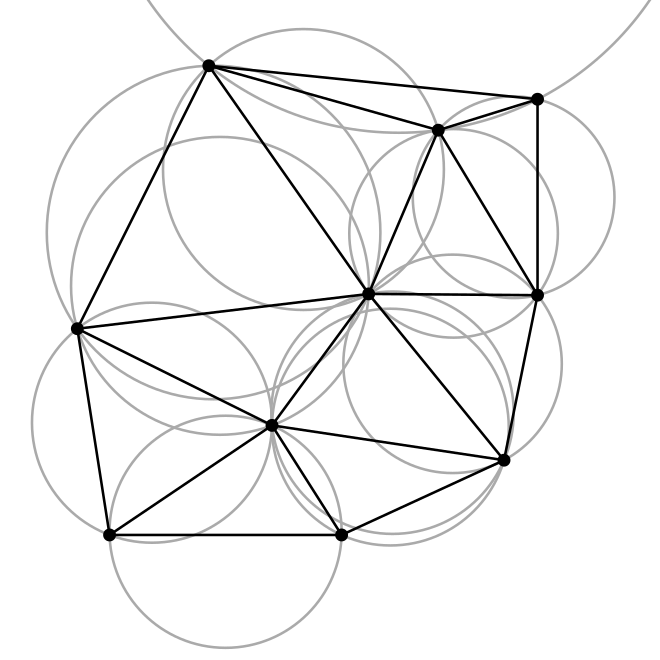
\includegraphics[width=2.5in]{images/illus_graphs/Delaunay_circumcircles_vectorial.svg.png}
    \caption{Example of a Delaunay triangulation}
    \label{del_tri}
\end{figure}

\subsection{Gabriel graph}
\noindent The Gabriel graph is a subgraph of a Delaunay triangulation. Thus, if the Delaunay triangulation is given, it can be found in a linear time. 

Gabriel graphs are named after K. Ruben Gabriel, who introduced them in a paper with Robert R. Sokal in 1969[citer].

Formally, it is the graph $G$ with vertex set $S$ in which any two distinct points $p\in S$ and $q\in S$ are adjacent precisely when the closed disc having pq as a diameter contains no other points.

\subsection{$k$-NN graph}
\noindent Nevertheless, the two methods presented above are triangulation, that is to say that they do not connect each \acrshort{bs} to all of its potential neighbours.

One simple idea to get rid of this problem could be solved by connecting each \acrshort{bs} to its $k$ nearest neighbours.

\section{Finding the real neighbours}

\noindent Each of the precedent methods gives us a list of potential neighbours for each \acrshort{bs}. However, we know that some of this neighbouring connexions are wrong,
because some \acrshort{bs} will be \og hidden\fg{} by others.

Thus, we need to find methods to suppress bad connexions. That was made by Delphine.

The main innovation of our work is to take in account the difference of \acrshort{bs}'s density.

\subsection{Measurement of \acrshort{bs} density}
\noindent To simplify the explanation, and because it is related, we will assume that solving this problem is equivalent to finding the \acrshort{bs} situated in \og cities\fg{}.

\subsubsection{DBScan}

\subsubsection{HDBScan}

\subsubsection{$3$-NN mean distance}
One provider $\gamma$

To classify each base station we need a method. Here, we will take the mean distance to the 3 nearest neighbours.

Let's call this value $\gamma$, in $\unit{km}$. So, we have 4 different categories.
For each category, we will apply a different distance and angle criterion :

\subsection{Filtering criteria}

\begin{table}[!b]
    \centering
    \caption{Summary of criteria values}
    \label{crit_summary}
    \begin{tabular}{clcc}
        \toprule
        \textbf{$\gamma$} & \textbf{Description} & \textbf{max\_distance} & \textbf{min\_angle} \\
        \cmidrule(lr){1-4}
        $\left[0, 1\right]$ & city center & $\unit[2]{km}$ & $5^\circ$ \\
        $\left]1, 2\right]$ & urban area & $\unit[5]{km}$ & $10^\circ$ \\
        $\left]2, 4\right]$ & extra-urban area & $\unit[10]{km}$ & $15^\circ$ \\
        $\left]4, \infty\right[$ & courntryside & $\unit[15]{km}$ & $20^\circ$ \\
        \bottomrule
    \end{tabular}
\end{table}

\begin{figure}[!t]
    \centering
    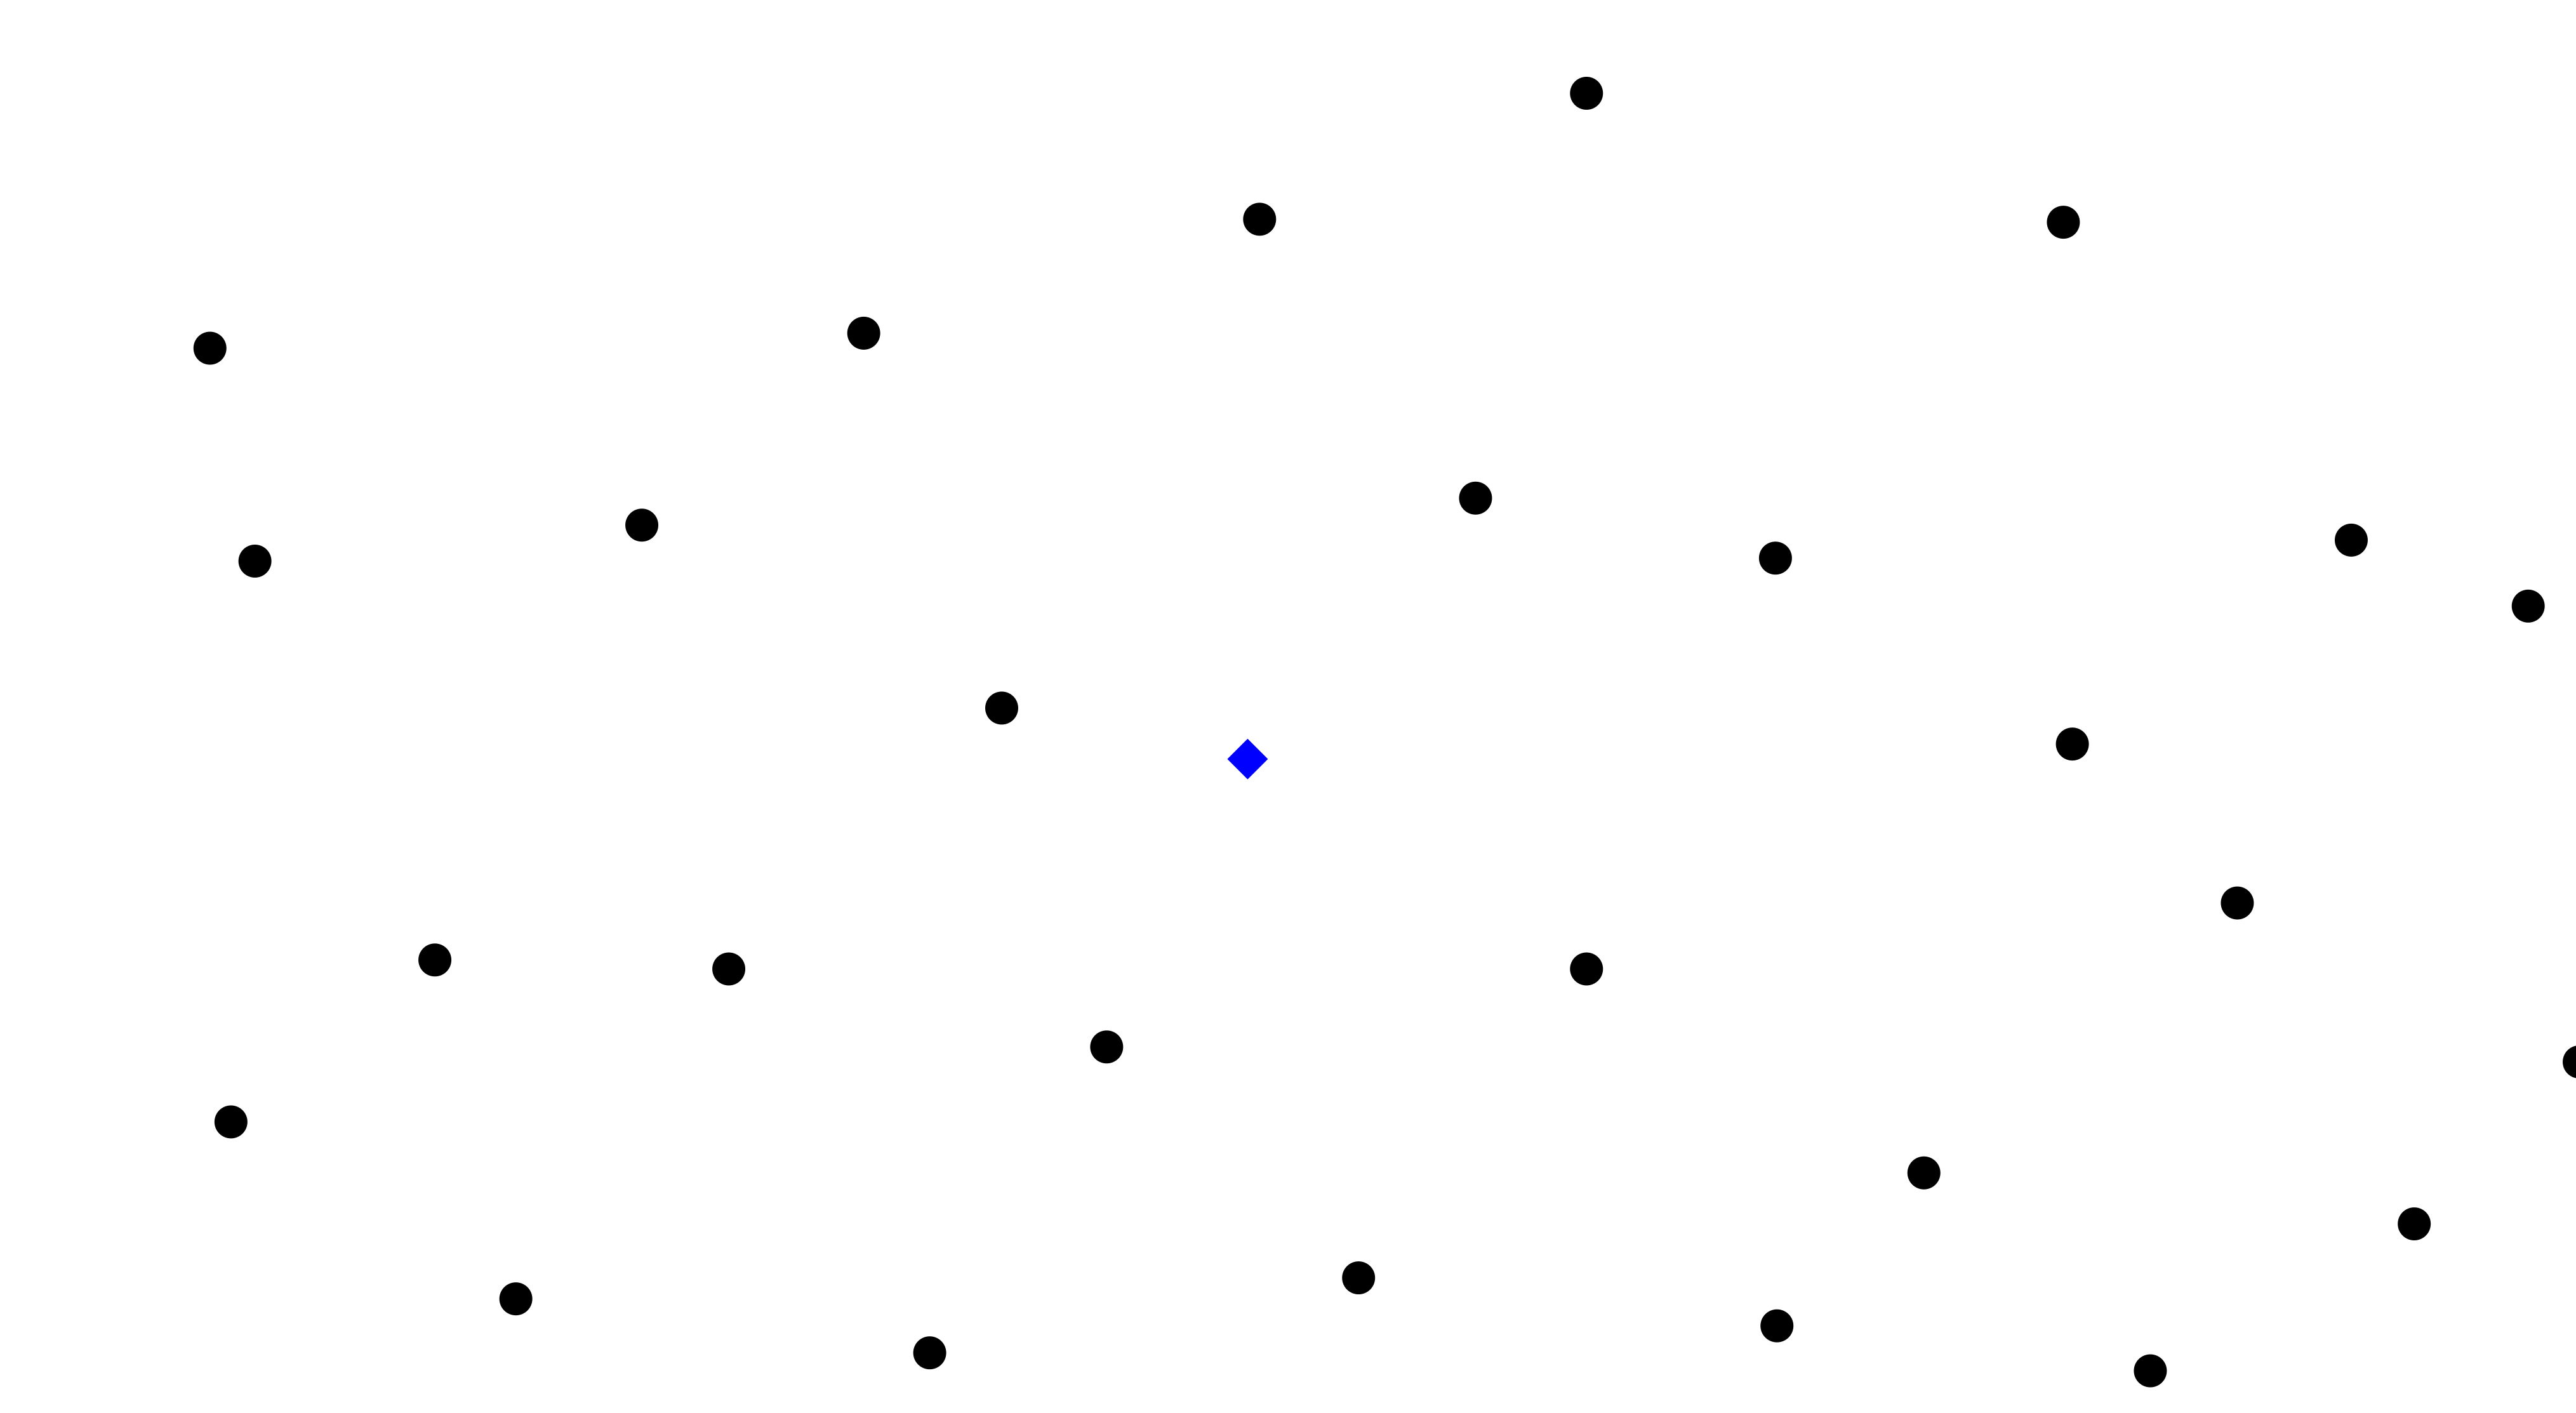
\includegraphics[width=2.5in]{images/illus_crit/points.png}
    \caption{Example of a Delaunay triangulation}
    \label{crit_pts}
\end{figure}

\begin{figure}[!b]
    \centering
    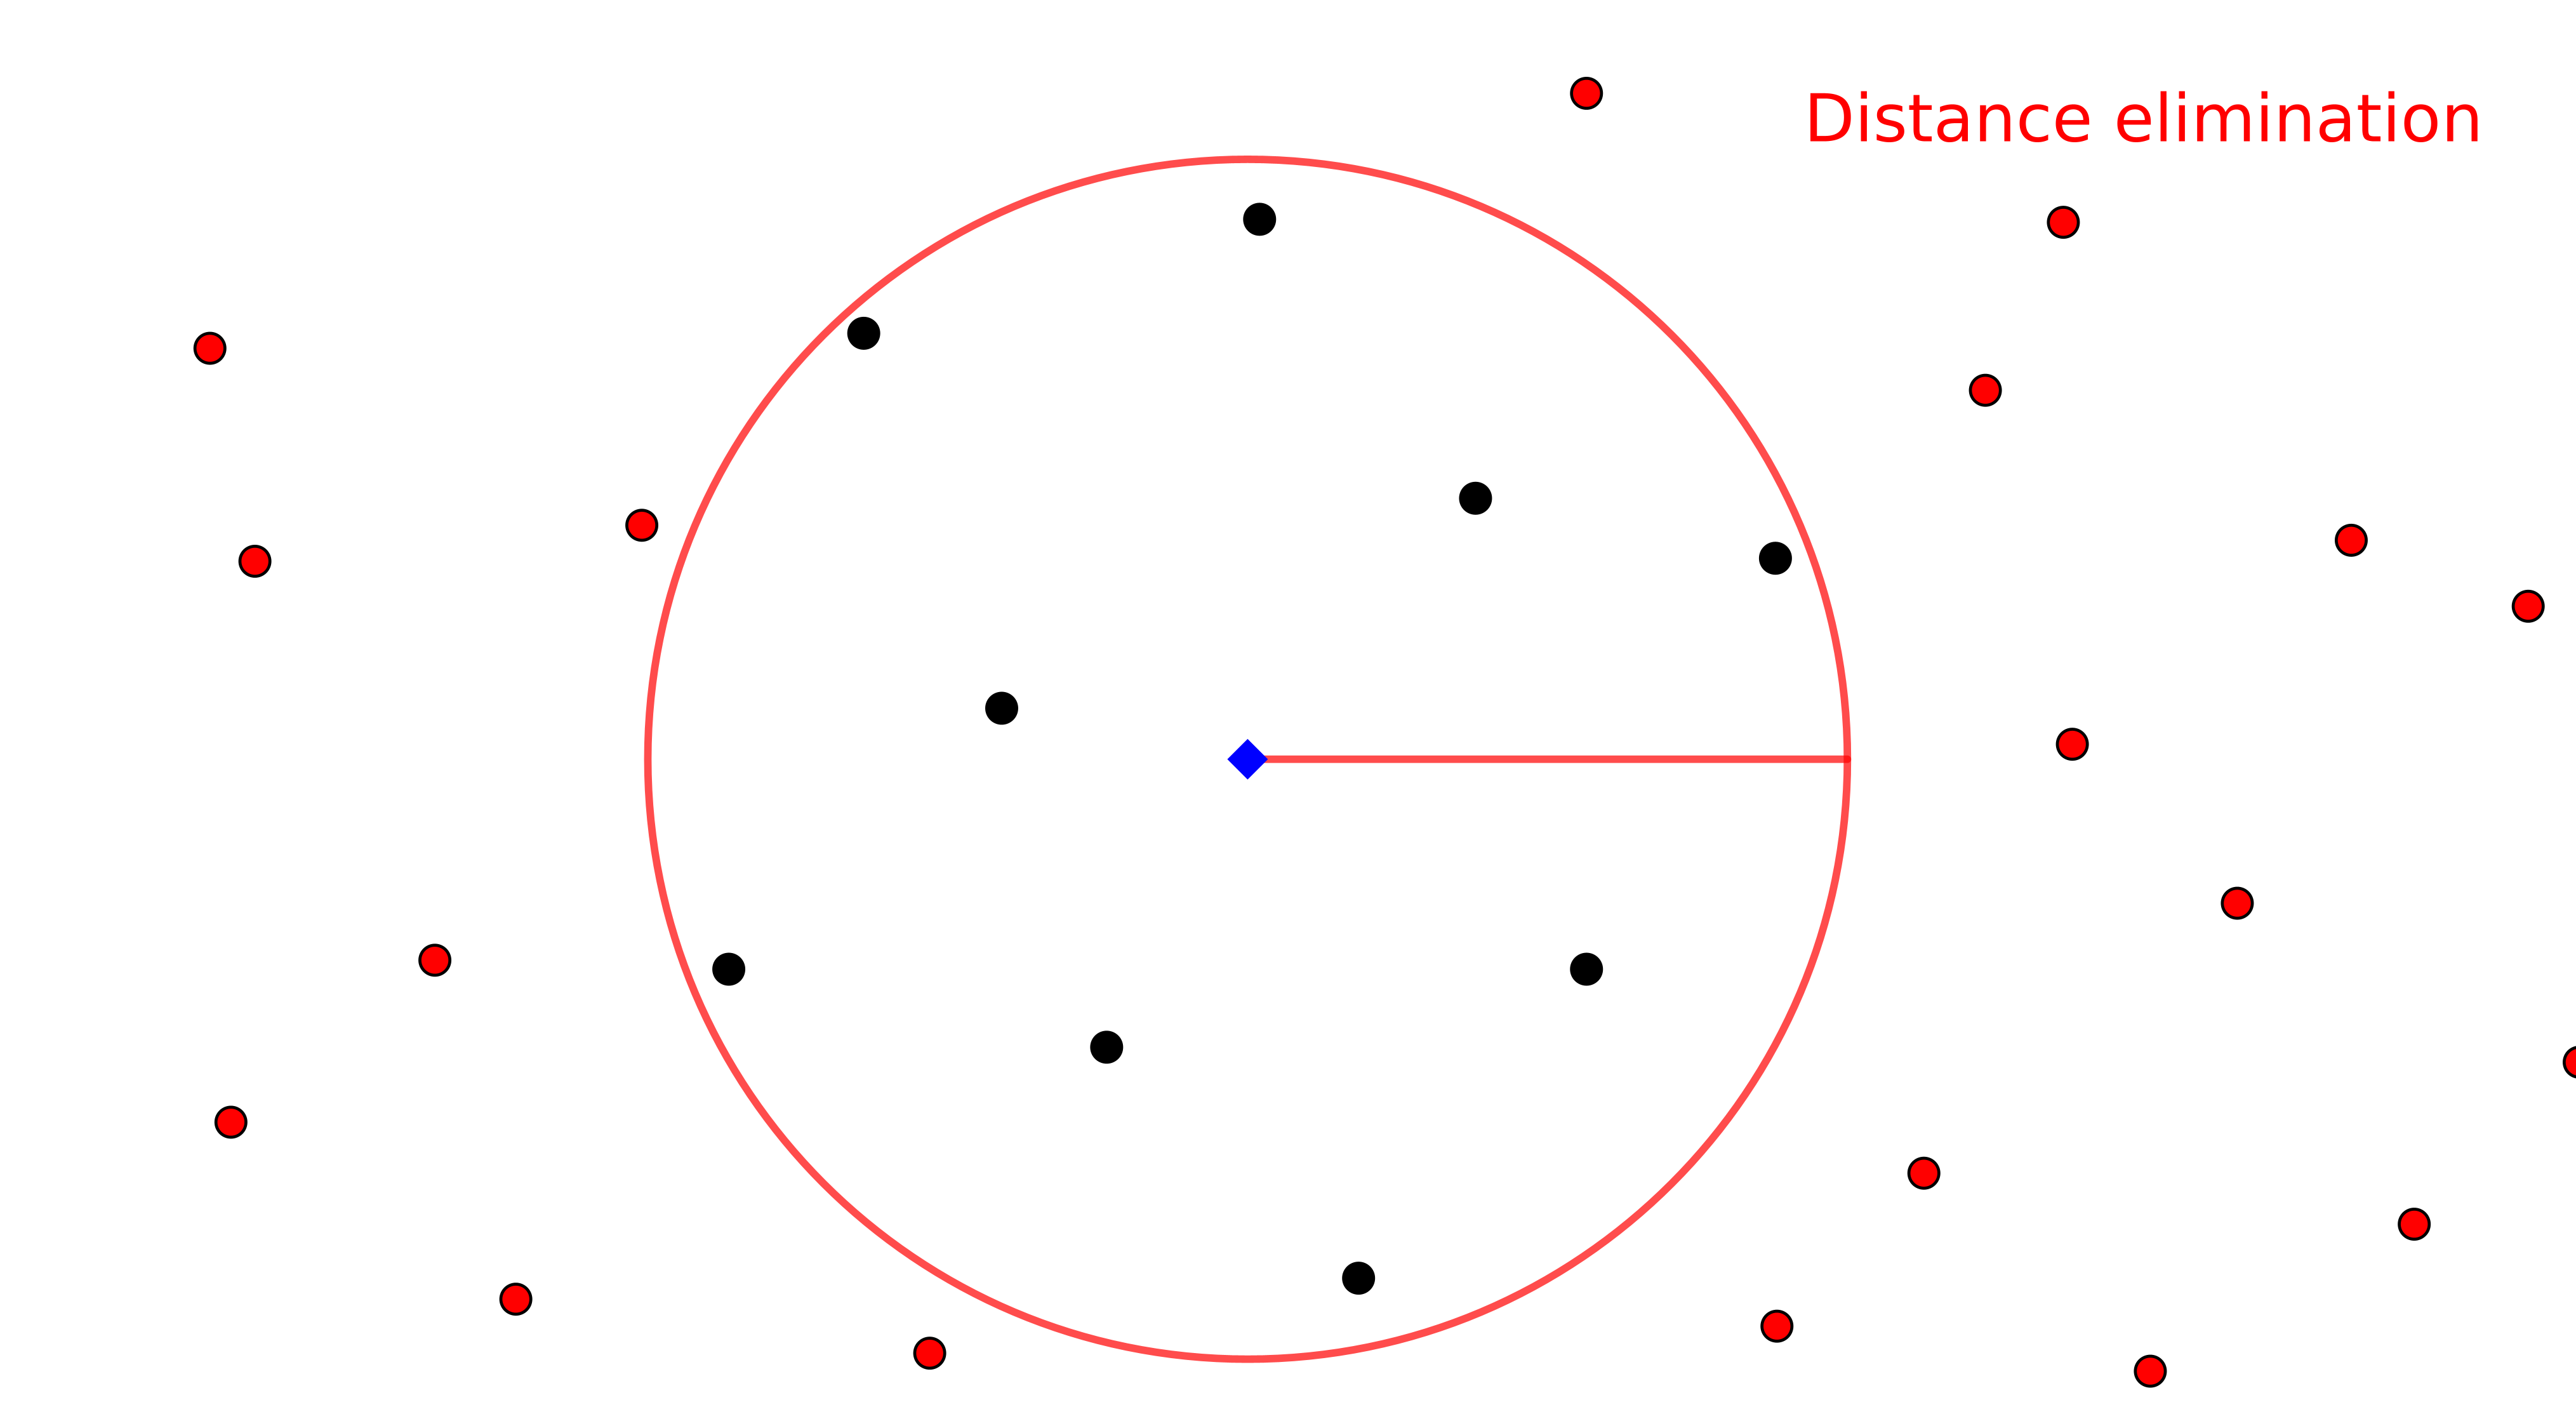
\includegraphics[width=2.5in]{images/illus_crit/distance_elim.png}
    \caption{Example of a Delaunay triangulation}
    \label{crit_dis}
\end{figure}

\begin{figure}[!t]
    \centering
    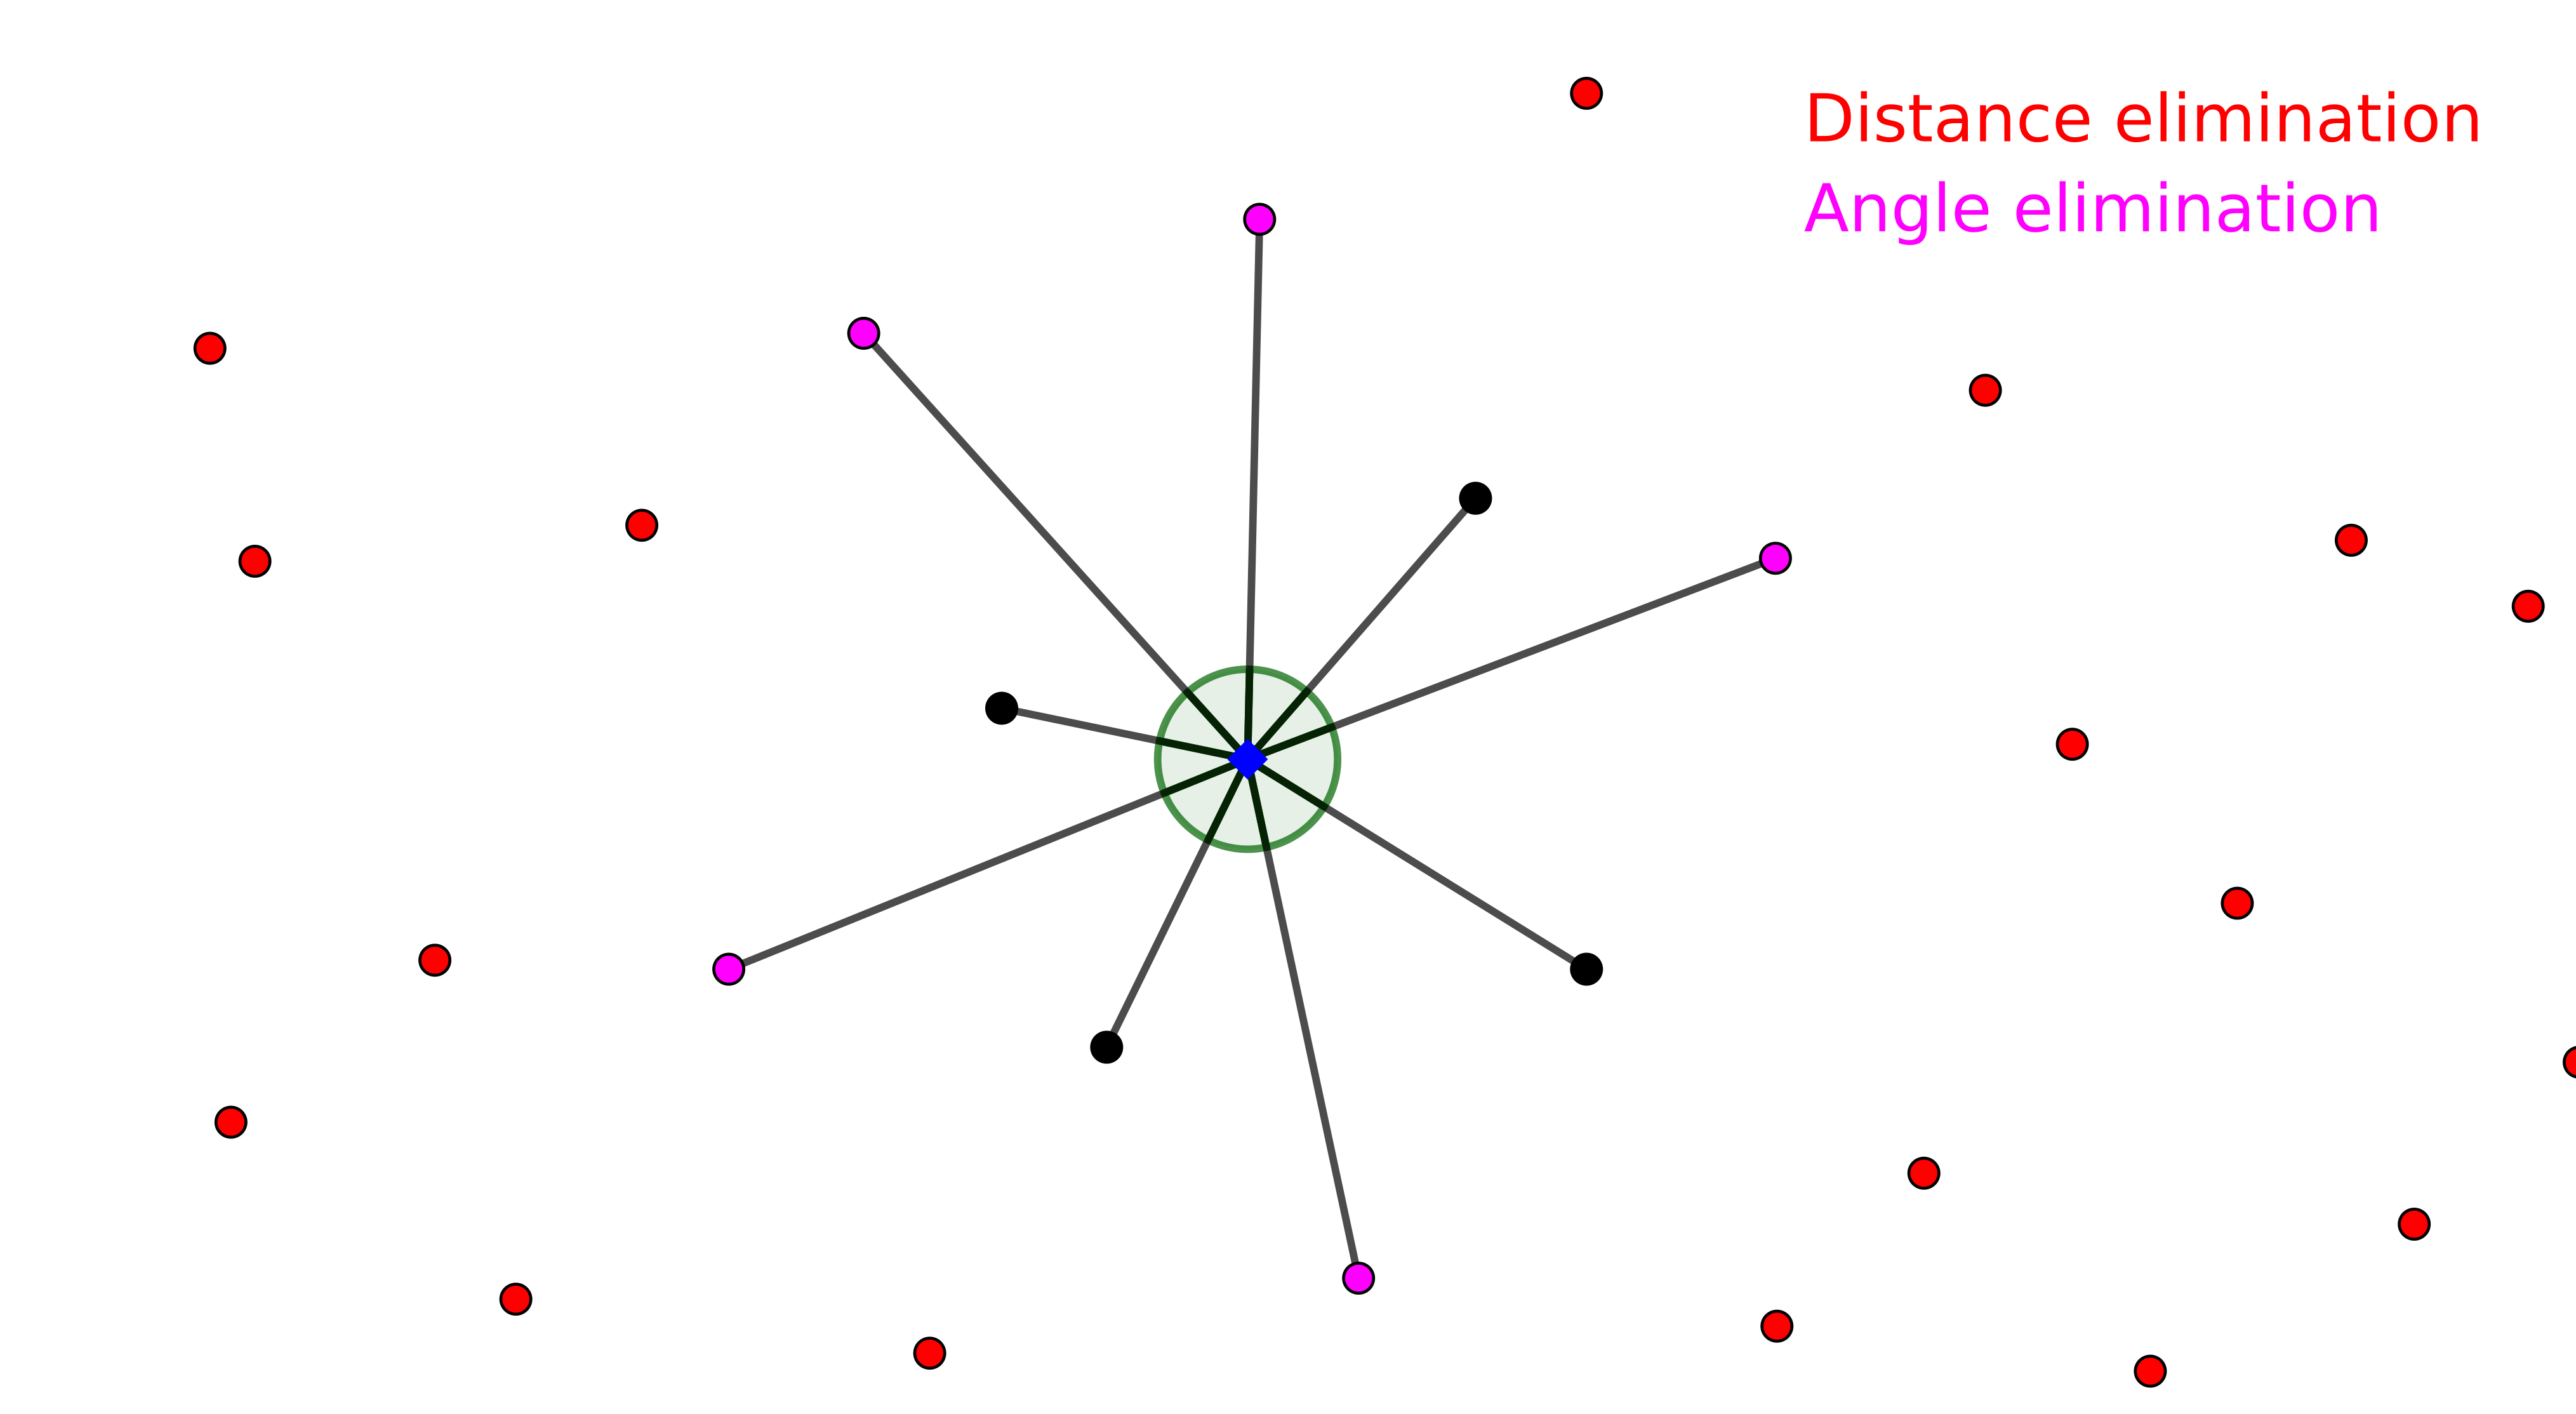
\includegraphics[width=2.5in]{images/illus_crit/angle_elim.png}
    \caption{Example of a Delaunay triangulation}
    \label{crit_ang}
\end{figure}

\begin{figure}[!b]
    \centering
    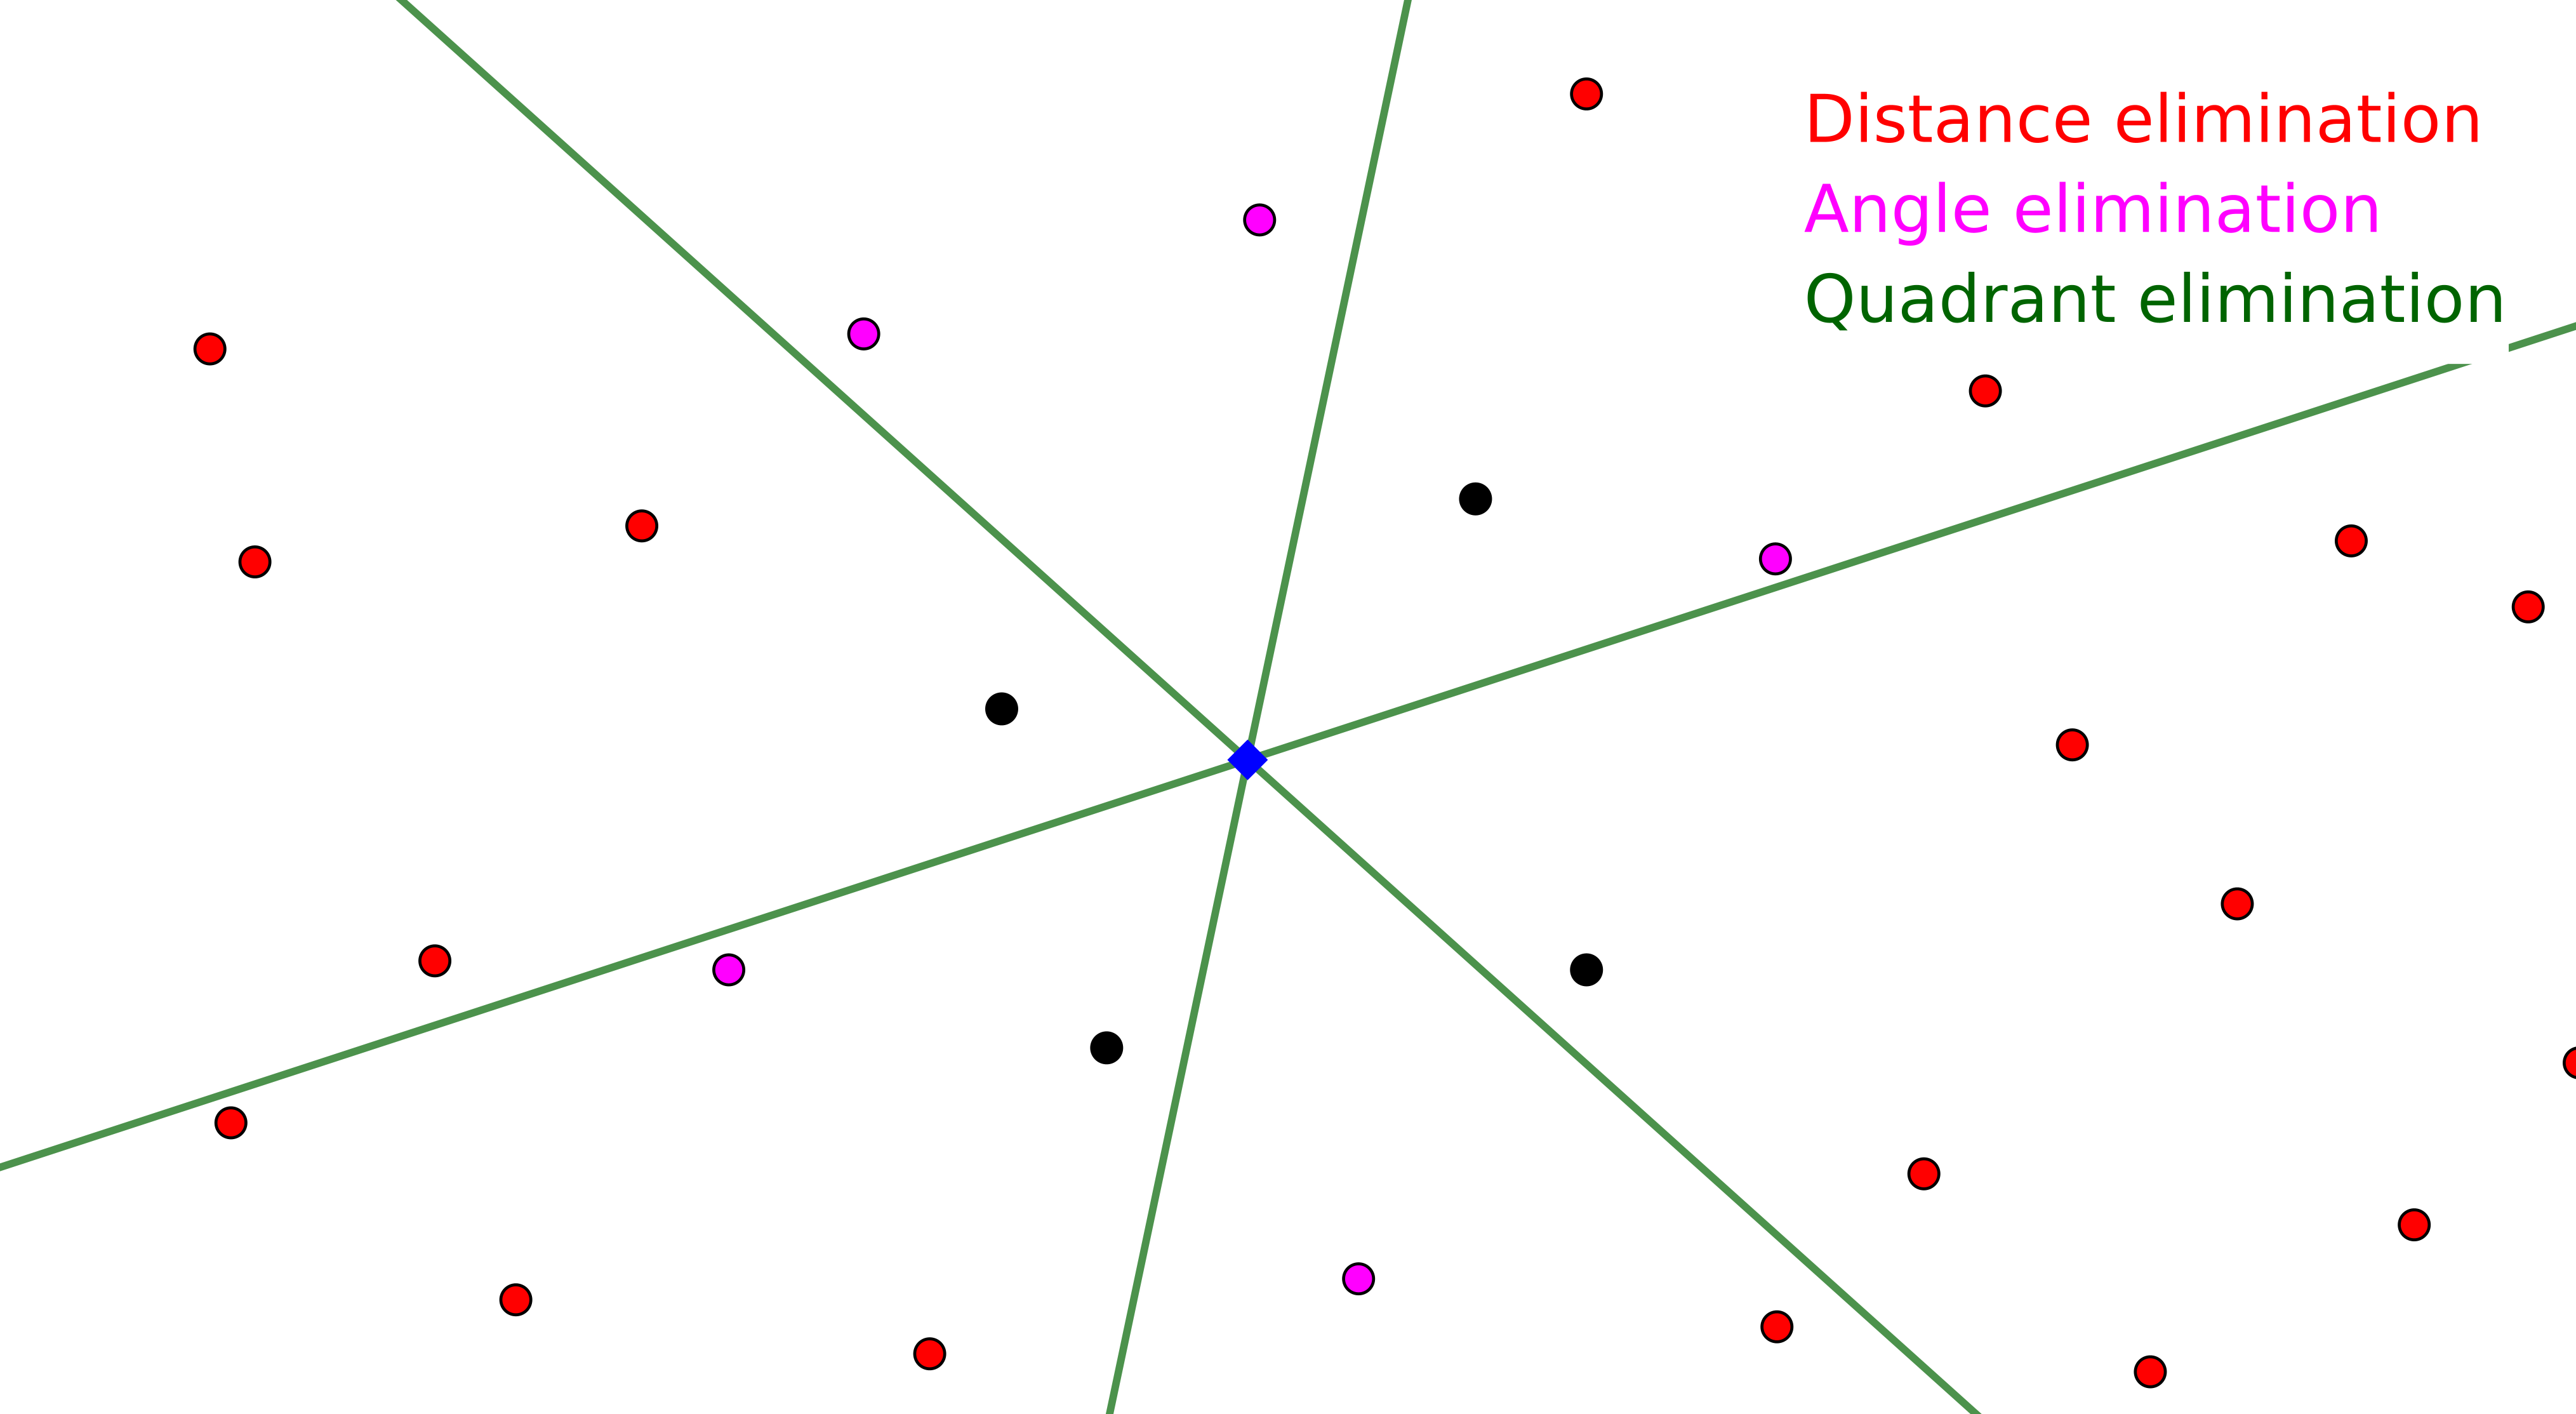
\includegraphics[width=2.5in]{images/illus_crit/quadrant_elim.png}
    \caption{Example of a Delaunay triangulation}
    \label{crit_qua}
\end{figure}

\begin{figure}[!t]
    \centering
    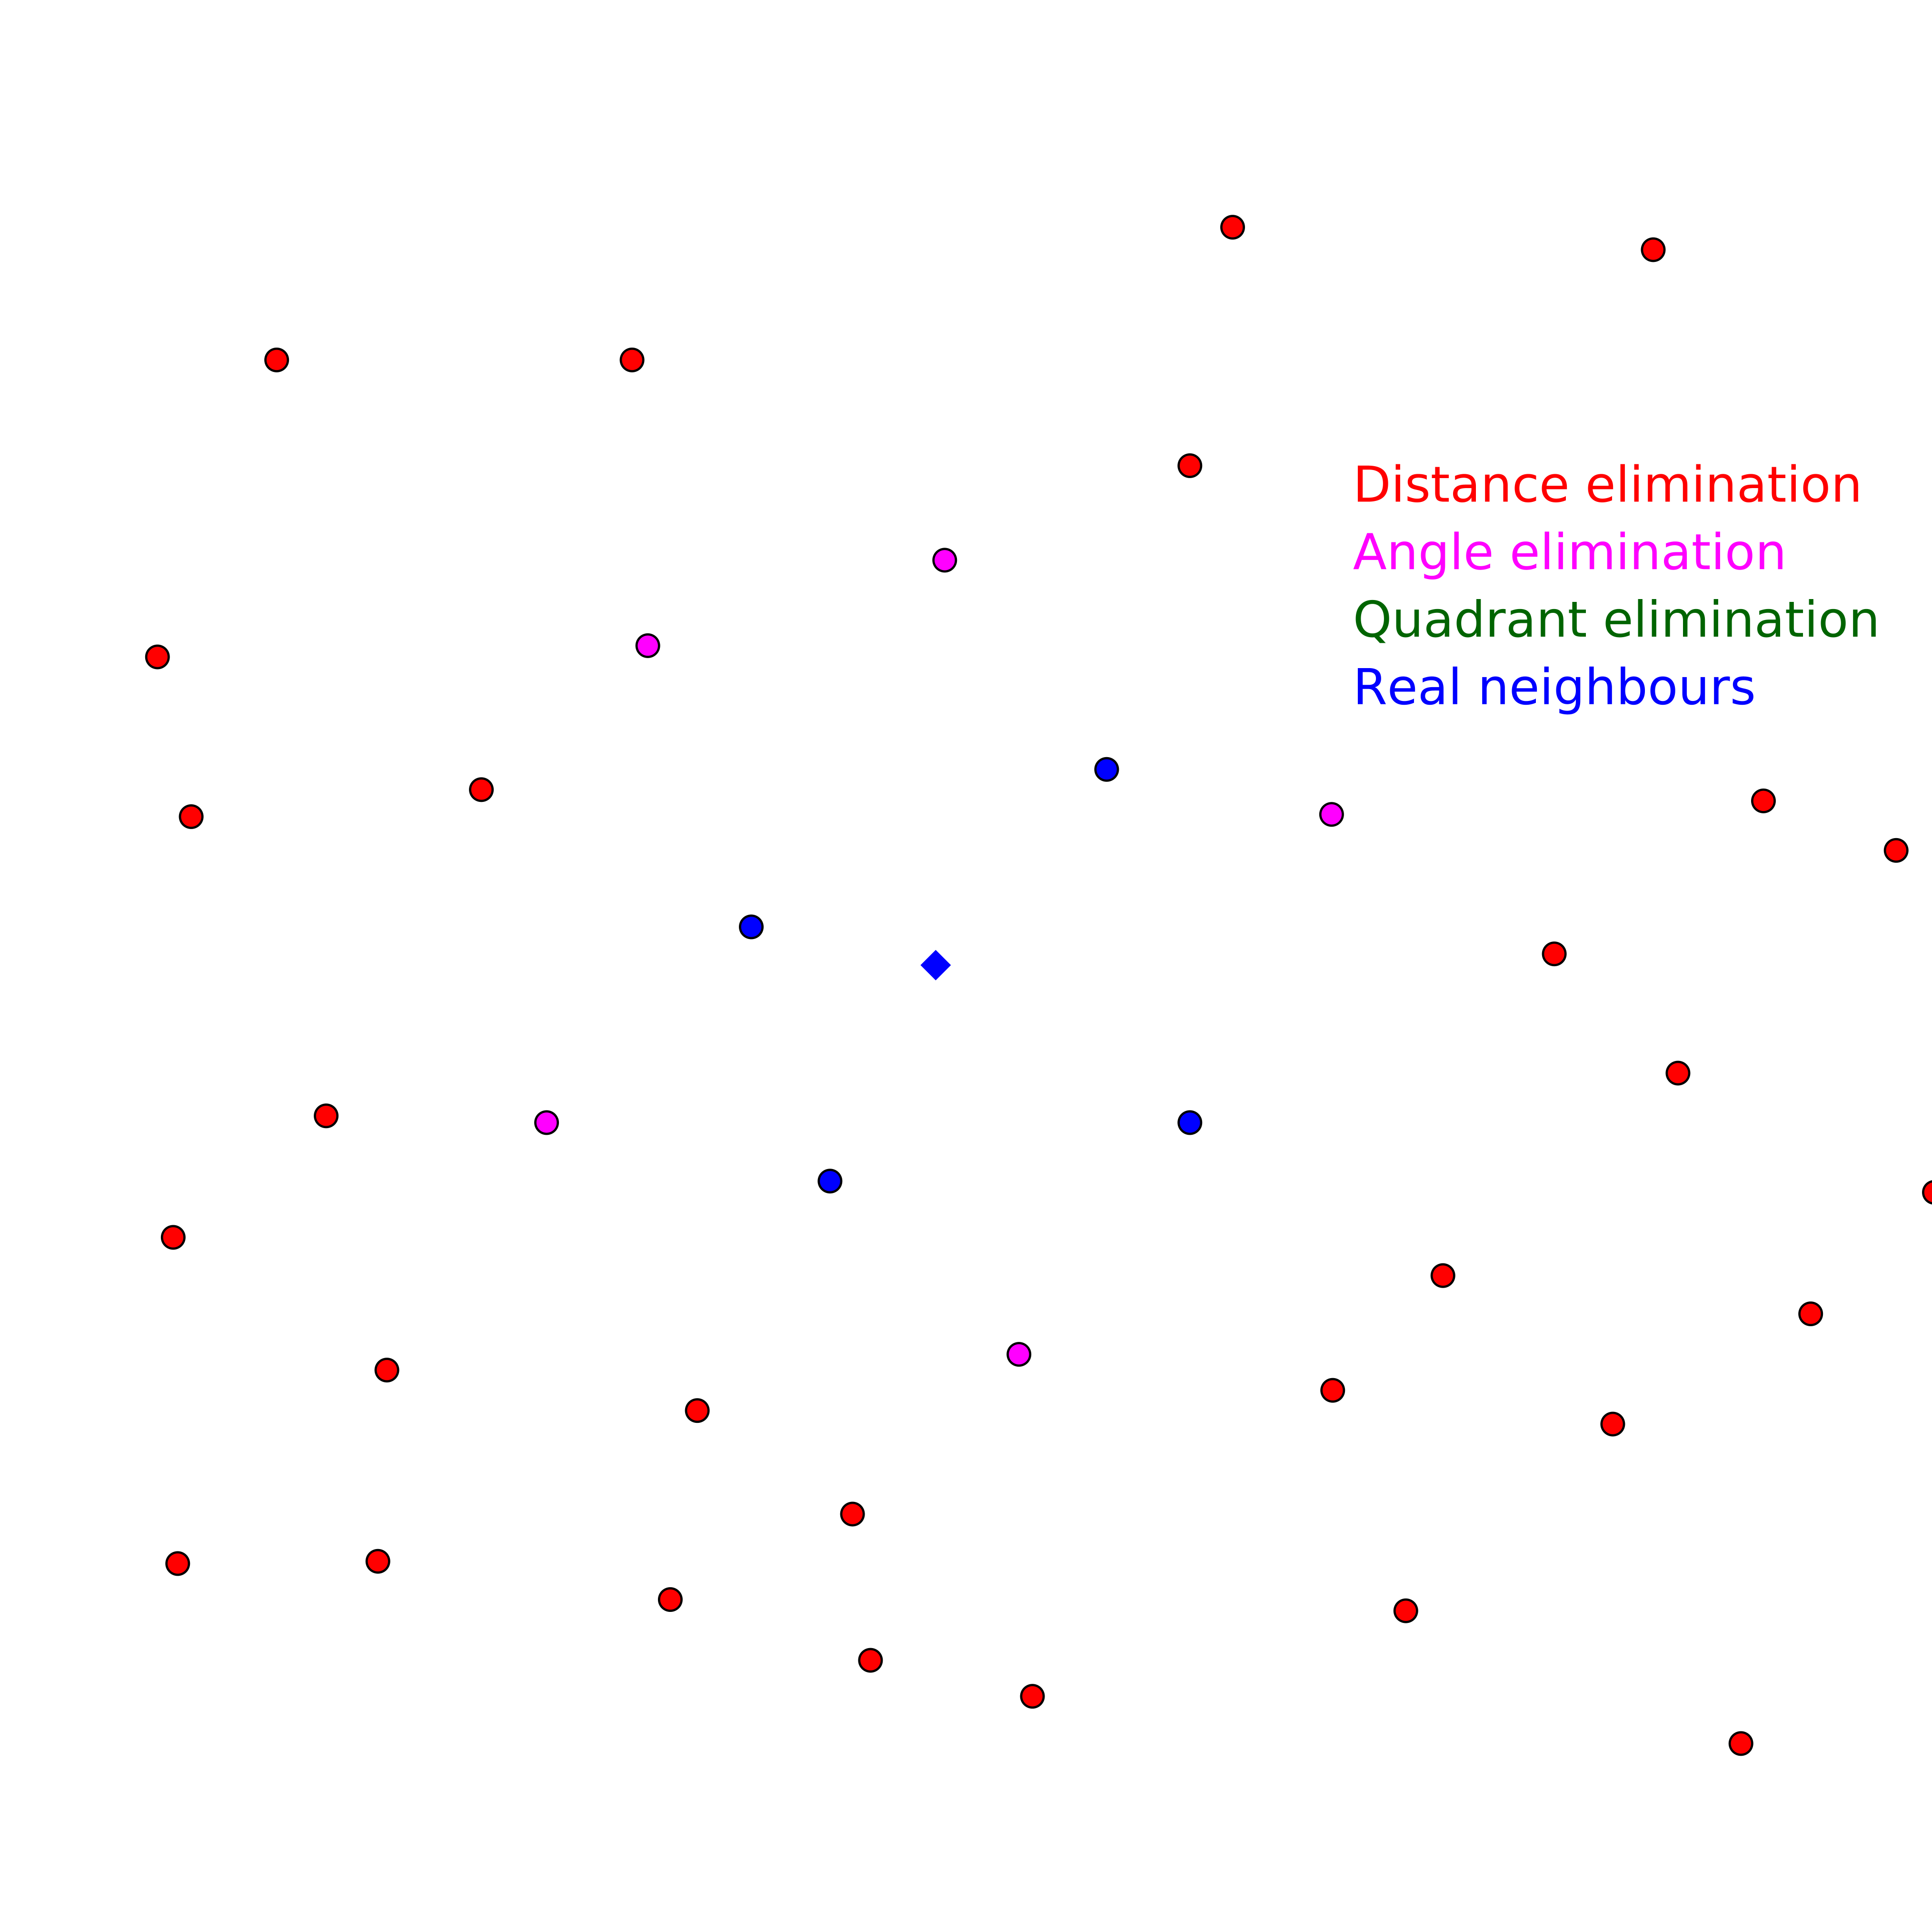
\includegraphics[width=2.5in]{images/illus_crit/neighs.png}
    \caption{Example of a Delaunay triangulation}
    \label{crit_nei}
\end{figure}

\subsubsection{Distance criterion}
Each \acrshort{bs} has its proper coverage area, which is not infinite. As a matter of fact, we need to suppress longer edges.

\subsubsection{Angle criterion}
For each \acrshort{bs}, we 

\subsubsection{Quadrant criterion}

\section{Results}

\section{Conclusion}

[Ouverture : prendre en compte les zazimuths]

\printglossary[type=\acronymtype]

\bibliographystyle{alpha}
\bibliography{./biblio.bib}

\end{document}


